\chapter{Theory and methods}
The two key areas of this project cover two widely different fields; 
crystallisation theory, which is covered in the previous introduction 
section, and tweezing theory. The following chapter summarises the 
working principles behind optical tweezing, the work being done with 
optical tweezers in particle classification, and how tweezing has been 
used to investigate nucleation events. 

\section{Working Principle}
Optical tweezing operates on the principle that light carries both linear and angular momentum, which can be transferred to other objects. If light is reflected or refracted by a medium part of the light's momentum is transferred to the medium itself. While at large scales this effect is insignificant in most cases, at micron scales the forces imparted by individual photons begin to become significant enough to influence its trajectory. Ashkin's work into optical tweezing found that micron sized entities could be spatially locked by aiming a laser with a Gaussian intensity profile directly upward at a the cell while being suspended in a liquid medium \cite{Ashkin1970}. This is demonstrated diagram below where we have a simple sphere trapped by a Gaussian beam, if we consider two rays of light hitting our sphere we see that while in the centre each ray is refracted in an equal opposite direction to one another and so the net force imparted is 0. However when displaced the net force is unbalanced and points towards the centre of the trap; this principle can be generalised to 3 degrees of freedom if we consider a focused beam instead of a para-axial beam, typically the trap will be weaker along the beam axis compared to the transverse trap strength.  

\begin{figure}[h]
	\centering
	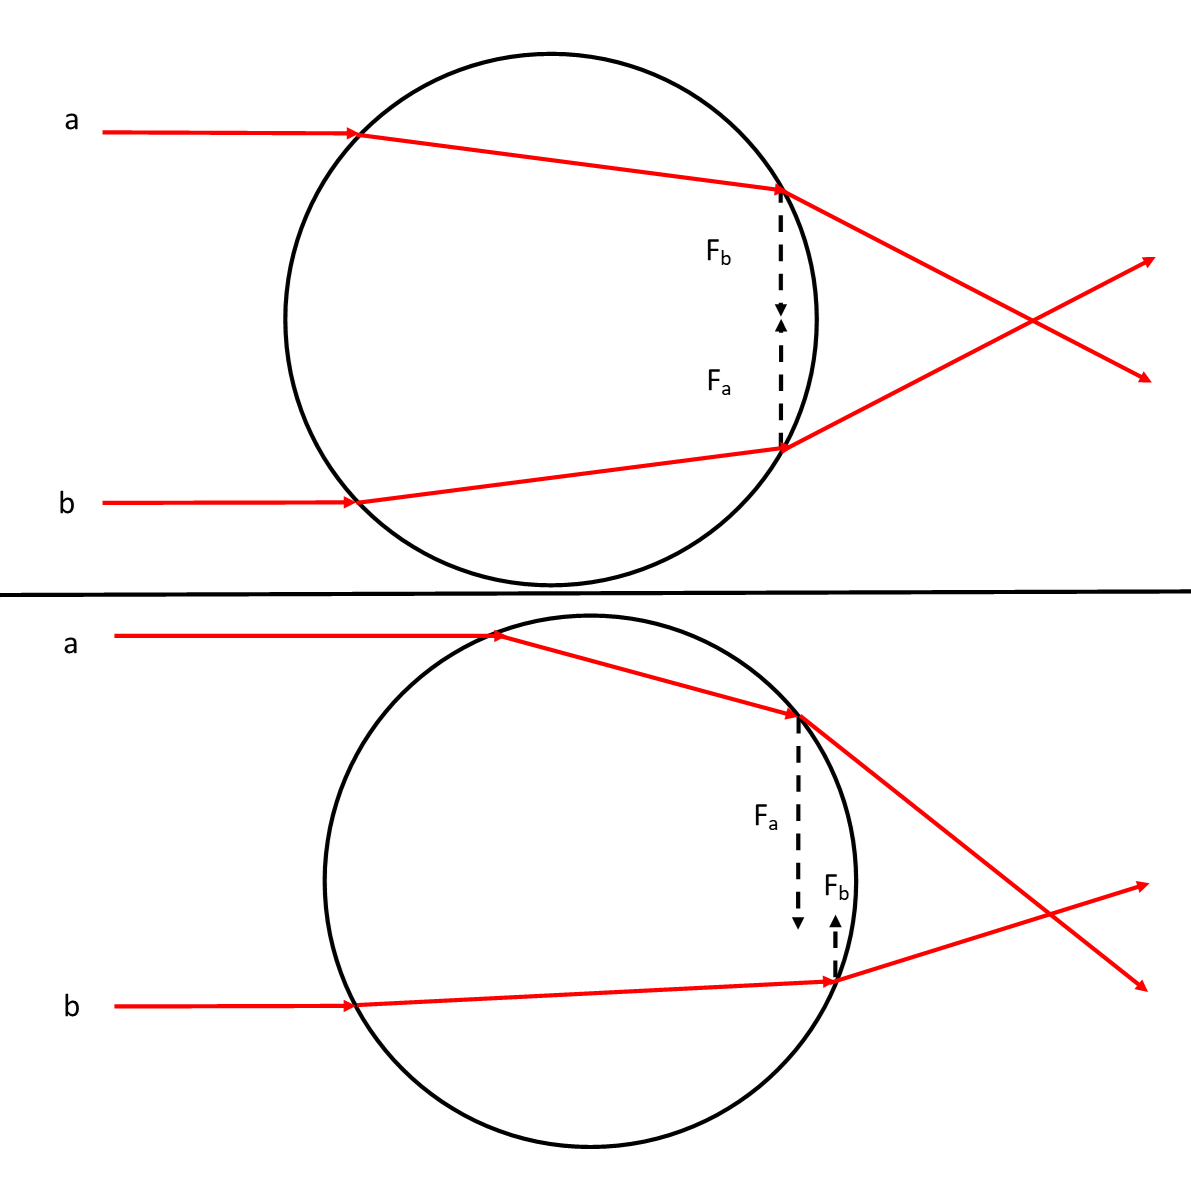
\includegraphics[width=0.65\linewidth]{ot_working_principal.png}
	\caption{Working principle for an optical trap, upper image shows a sphere at the centre of a trap experiences equal forces directed towards inwards. Lower image shows that when displaced 'ray a' is refracted far more than 'ray b' resulting in a net force back towards the centre.}
\end{figure}

\section{Electromagnetism and optical tweezing}
Proper understanding of optical tweezing requires an understanding of how the trapped particle interacts with the trapping laser. From a electromagnetism perspective the laser creates a spatially and temporally coherent electric field that scatters light off of a trapped particle. The laws governing electric and magnetic fields are summarised most succinctly via the Maxwell equations. The differential forms of which are given below:
\begin{align}
	&\nabla \cdot \mathbf{E} = \frac{\rho_ v}{\epsilon_0} \\
	&\nabla \cdot \mathbf{B} = 0 \\
	&\nabla \times \mathbf{E}  = \frac{\delta \mathbf{B}}{\delta t} \\
	&\nabla \times \mathbf{B} = j_0 +\frac{\delta \mathbf{E}}{\delta t}    
\end{align}
These 4 equations describe how the electric and magnetic fields must behave and are also related to one another, any discussion of optical trapping is underpinned by the fact that in all cases the Maxwell Equations must be satisfied. 

The force exerted by an optical tweezer can be subdivided into the gradient and scattering components, for most modelling research this is how the force fields are reported. The gradient force is a conservative force brought about by the polarisation of dielectric materials, anything around 10\% of the trapping wavelength will be attracted along the gradient of the electric field to the region of greatest intensity (for a simple Gaussian Beam this would be at the focal point). The scattering force arises from the scattered field of the trapping beam pushing the target object away from the focal point; unlike the gradient force, the scattering force is non-conservative and is loosely proportional to the particle's Brownian motion. The equilibrium position (where the mean squared displacement is minimised) is found when the gradient force far exceeds the scattering force, interpreting and calculating these forces is dependent on the ratio between the particle size and the trapping wavelength.

\subsection{Ray-Optics Regime}
The Ray-Optics model is the simplest to understand, the theory models the laser as a collection of individual 'rays' that propagate and are refracted according to Snell's Law. Based on the change in direction momentum is transferred to the target particle; with rays closest to the centre of the beam having greater intensity than those rays at the very edge of the beam. Consider a particle struck by two rays in a Gaussian beam (see Fig below), one coming close to the centre, and the other ray coming from the edge. As each ray is refracted by the target sphere a force is imparted onto it, the total force imparted is given by:

\begin{align}
	F_i = Q_i\frac{\Delta n P_i}{c}
\end{align}

Where $Q_i$ is the trapping efficiency, $\Delta n$ is the difference in refractive indices between the solution and the target particle, and $P_i$ is the power of the individual ray. For a beam with a Gaussian intensity distribution $P_i$ will fall off as you move from the centre of the beam. The ray optics model is ideal for  

\subsection{Lornez-Mie Theory}
The Lorenz Mie theory provides an exact solution to the maxwell equations for the scattering caused by an isotropic sphere. The theory describes the scattered wave given off by a dielectric sphere when incident by a plane wave as a summation of partial spherical waves. For any spherical wave the vector fields must solve the Helmholtz wave equation given by:
\begin{align}
	\nabla^2\mathbf{E} +k^2\mathbf{E} = 0
\end{align} 
This combined with the constraints of Maxwell's Equations leaves very few exact solutions apart from spherical or planar waves, both of which can be converted between with relative ease. For example, a plane wave electric field can be expanded into spherical harmonics and likewise any spherical wave can be described as combination of plane waves offset from one another. For a single plane wave the incident, internal, and scattered fields are given as:

\begin{align}
	E_{inc}(r) &= E_0 \sum_{n=1}^\infty a_{n}M_{1n}^{(1)}(r)+b_{n}N_{1n}^{(1)}(r) \\
	E_{int}(r) &= E_0 \sum_{n=1}^\infty i^n\frac{2n+1}{n(n+1)}\left(-id_{n}N_{1n}^{(1)}(r)+c_{n}M_{1n}^{(1)}(r)\right) \\
	E_{scat}(r) &= E_0 \sum_{n=1}^\infty  i^n\frac{2n+1}{n(n+1)}\left(-ip_{n}N_{1n}^{(3)}(r)+q_{n}M_{1n}^{(3)}(r)\right)
\end{align}

Where $a_n$, $b_n$, $c_n$, $d_n$, $p_n$, and $q_n$ are the expansion coefficients of each of the fields, for the incident field computing its expansion coefficients is possible via analytical methods and are completely dependent on the beam conditions imposed by the user. However, computing the expansion coefficients of the internal and external fields be far more tedious depending on the shape of the target and what properties of the scattered field are desired - all of which is discussed later on. From an optical trapping perspective the force exerted by a focused electric field can be found by computing the maxwell stress tensor which only requires the total magnitude of the incident and scattered fields, essentially computing the momentum contained in the incident beam and how much of it has been transferred to the target particle. 

Lornez-Mie theory can be applied to describe the scattering from any particle regardless of size, however as we either increase or decrease the size of the target particles the infinite series converges allowing one to ignore much of the tedium of Lorenz-Mie theory. The ray optics model is what is achieved when the size of the target particle far exceeds that of the laser wavelength and thus individual ray's can have independent contributions. In the latter case we can simplify the scattering problem by approximating our target as a single dipole, focusing only its interactions with the incident field.

\subsection{Rayleigh Regime}
The Rayleigh approximation is the limiting approximation for describing a particles motion in an electromagnetic field who's wavelength is several times greater than the particle's size. The underlying theory is that a dielectric sphere can be treated as a dipole while in the presence of the electromagnetic field; in which case the scattering force is given simply by the scattering of the induced dipole, and the gradient force is due to the Lorentz force \cite{Gordon1973}. The gradient forces in the principle Cartesian axis are described by Harada et al \cite{YasuhiroHarada1996} in MKS units as a restorative rectangular force field:

\begin{align}
	F_{grad,x} &=-\hat{x} \frac{2\pi n_2 a^3}{c}
	\left(\frac{m^2-1}{m^2+2}\right) \frac{4\tilde{x}/w_0}{1+(2\tilde{z})^2} \times I(r) \\
	F_{grad,y} &=-\hat{y} \frac{2\pi n_2 a^3}{c}
	\left(\frac{m^2-1}{m^2+2}\right) \frac{4\tilde{y}/w_0}{1+(2\tilde{z})^2} \times I(r) \\
	F_{grad,z} &=-\hat{z} \frac{2\pi n_2 a^3}{c}
	\left(\frac{m^2-1}{m^2+2}\right) \frac{4\tilde{y}/w_0}{1+(2\tilde{z})^2} \nonumber \times I(r) \\ 
	& \times \left[1-\frac{2(\tilde{x}^2+\tilde{y}^2)}{1+(2\tilde{z})^2} \right] \\
	\text{where:} \nonumber \\
	I(r) &= \left(\frac{2P}{\pi w_0^2}\right) \frac{1}{1+(2\tilde{z}^2)} 
	exp \left[ - \frac{2(\tilde{x}^2+\tilde{y}^2)}{1+(2\tilde{z})^2} \right]
\end{align}

Where $m$ is the relative refractive index ($n_1/n_2$), $\omega_0$ is the beam waist, and $a$ is the radius of the particle. Scattering force however is dependent on the effective scattering cross sectional area. 

\begin{align}
	F_{scat} &= \hat{z} \left(\frac{n_2}{2}\right) C_{pr} I(r) \\
	\text{where:} \nonumber \\
	C_{pr} &= \frac{8}{3} \pi (ka)^4 a^2 \left(\frac{m^2-1}{m^2+2}\right)^2
\end{align}

The Rayleigh regime allows for easy computation of the gradient and scattering forces due to the assumption that the particle is a point dipole, so much so that higher order scattering problems can be simplified by subdividing the particle into discrete dipoles (see Sec \ref{sec:scattering}). However as the target particle gets larger this assumption fails to accurately describe the trapping force due to the complexity in the gradient field. For particle sizes close to the laser wavelength the scattered field is best described by Lorenz-Mie theory. 

\section{Scattering methods}
\label{sec:scattering}
\subsection{Tmatrix}
The T matrix method was first developed by Peter Waterman with his 
research into acoustic wave scattering, this would later be extended to 
electromagnetic waves. Put simply, the method sets a boundary condition 
where the incident field within the interior field is cancelled out via 
interference; these boundary conditions allows us to solve the Maxwell 
equations by expanding the incident and scattered fields using spherical 
vector waves. Because the boundary condition ensures that the incident field is halted at the interior surface of the object, the scattering field can be related to the incident field by the objects T-Matrix:

\begin{align}
	\begin{pmatrix}
		q_{mn} \\
		p_{mn} 
	\end{pmatrix}
	= \bold{T} 
	\begin{pmatrix}
		a_{mn} \\
		b_{mn}
	\end{pmatrix}
	= \begin{pmatrix}
		T_{11} \ T_{12} \\
		T_{21} \ T_{22}
	\end{pmatrix}
	\begin{pmatrix}
		a_{mn} \\
		b_{mn}
	\end{pmatrix}
\end{align}

The T-matrix method is exceptionally useful for computing the scattering from any arbitrary shaped particle. However, the T-matrix method by itself can be limited by computation power for aggregates of particles; while possible to compute the scattering of each individual particle the system of equations cannot be solved analytically and must be solved numerically to determine properties for the aggregate for one particular orientation. 

\subsection{Discrete Dipole Approximation}

\section{Langevin Equation}
Describing any microscopic motion requires an understanding of a molecules diffusive behaviour, for the case of optical tweezers the most complete model of diffusion is the Langevin equation. Models such as the Fickian, and Einstein derivations are sufficient for macroscopic behaviours the Langevin equation better describes the microscopic characteristics of any diffusive behaviour. The Fickian model is not suitable for the applications of optical tweezers as it assumes that all diffusive motion is driven by a gradient of molecular density, not only is this often not the case but it fails to describe the motion of any single molecule, only the collective behaviour. Einstein's model however considers the collisions experienced by individual molecules, if we assume that all collisions are random and only consider the behaviour after a finite time step $\delta t$ then the individual collisions should cancel out. This is insufficient for our interests as an optical tweezers relaxation time (given by $\tau = \kappa/\gamma$) is often so short that we must consider the individual collisions experienced by any one molecule. The Langevin model of diffusion therefore assumes that the net force on a particular particle is described fully by these individual collisions:
\begin{align}
	m\frac{dv}{dt} + \gamma_0 v + F(t) = W(t)
\end{align}
Where the first term accounts for inertial forces, the second term accounts for friction forces which counteract the particles current motion ($\gamma_0$ is the friction coefficient), and the final term accounts for the random Brownian force. The $F(t)$ is there for convention which accounts for any external forces acting on the particle. We can say that the noise term $W(t)$ has a Gaussian probability, with a correlation function of:

\begin{align}
	&W(t) = \sqrt{2k_BT\gamma_0}\eta(t) \\
	&\langle W_i(t)W_j(t')\rangle = 2k_BT\gamma_0\delta(t-t')
\end{align}

The Langevin model can be extrapolated to describe the diffusive behaviour of an overall system, but for this project we can instead consider the behaviour of some particle with a diffusion tensor $D$ suspended in a viscous fluid and spacially localised by an optical potential with trap strength $\kappa$. Assuming the only external force acting on our particle is the laser the net force should be exactly equal to force of the stochastic collisions due to the fluids thermal energy. If we focus our analysis when the particle is stably trapped and assume that the trap is harmonic we can model the trapping force as a Hookean spring ($F(t) \approx \kappa x(t)$). The full Langevin equation for an optically trapped particle is therefore given as:
\begin{align}
	\label{eq:langevin}
	m\frac{\delta^2x(t)}{\delta t^2} + \gamma_0 \frac{\delta x(t)}{\delta t} + \kappa_x x(t) = \sqrt{2k_BT}\eta(t)
\end{align}

Eq.~\ref{eq:langevin} provides an accurate description of strongly trapped particles, however the analytical solution of the Langevin equation requires integration of the white noise term making it difficult to simulate the trajectory of a given particle \cite{Volpe2013}. Instead it is often far easier to solve the equation numerically and apply use the analytical solution to calibrate and extract information about the particle and fluid, and how the two interact with the optical trap.

\subsection{Finite Difference}
The Finite Difference approach involves discretizing the time and spatial elements in order to approximate the higher order terms. If we assume that $x(t)$ is differentiable to n (we can find its $n^{th}$ derivative) then we can use the Taylor series expansion to get:
\begin{align}
	x(t+\Delta t) = x(t)+\frac{x'(t)}{1!}\Delta t + \frac{x^2(t)}{2!}\Delta t^2+...+\frac{x^n(t)}{n!}\Delta t^n+R_n(x(t))	
\end{align}
Where $R_n(x(t))$ is the remainder term between the Taylor expansion to term n and the actual expression. If we limit our approach to the first derivative only we find that for sufficiently small values of $R_1$ the velocity and acceleration can be approximated as:
\begin{align}
	x'(t) &= \frac{x(t+\Delta t)-x(t)}{\Delta t}=\frac{dx(t))}{dt} \\
	x^2(t) &= \frac{x'(t+\Delta t)-x'(t)}{\Delta t} = \frac{x(t)-2x(t+\Delta t)+x(t+2\Delta t)}{\Delta t^2}
\end{align}
By reversing the time step (i.e. use $-\Delta t$) to approximate the velocity and acceleration based on the previous time steps we can discretize the position by taking finitely small  time steps (i.e. $x(t) = x_i,\ x(t-\Delta t) = x_{i-1}$). The same cannot be done for white noise as no information is known about $W(t)$ at any time. We can instead say that the velocity of a Brownian particle should approximate our white noise as a random walk, where at each new time step the position changes randomly within a given range. Constricting the variance to $\sqrt{2D}/\Delta t$ allows us to represent the white noise using the finite-difference approach as:
\begin{align}
	m\frac{x_i-2x_{i-1}+x_{i-2}}{\Delta t^2} = -\gamma\frac{x_i-x_{i-1}}{\Delta t}+\sqrt{2k_BT\gamma}\frac{w_i}{\sqrt{\Delta t}}
\end{align}
Where $w_i$ is a random real number between -1 and 1, we can say that it is normally distributed around 0 for simulation purposes. We can rearrange this for $x_i$ to approximate the Brownian motion of a particle (setting $x_0=0$), where the characteristic time is $\tau = m/\gamma$. Now in the case of an optical trap the restoration time scale is given by $\tau_{OT}=\kappa_x/\gamma$ which for strongly trapped particles is far greater than the characteristic time, therefore for simulation purposes we can neglect the particle's inertia which allows us to write the motion of an optically trapped particle as:
\begin{align}
	\label{eq:sim_langevin}
	x_i = x_{i-1} + \tau_{OT}\ x_{i-1}\Delta t + \sqrt{2D\Delta t}\ w_i
\end{align} 

This result can be generalised for a 3-dimensional description of an optically trapped particle, where each Cartesian direction has its own unique characteristic restoration time. We see from the result that trajectory is dependent on only a handful of factors, the trap stiffness $\kappa_x$, the fluid viscosity $\gamma$, and the thermal energy of the system $k_BT$ - with the latter two being related by Einstein's formulation of the diffusion coefficient $D = k_BT/\gamma$. Therefore by calculating these parameters to a high degree of precision allows one to get precise description of the forces experienced by a target particle, which in the past has been used for highly accurate force transduction \cite{BergSoerensen2004, Smith2003}.

\section{Calibration Techniques}
\label{sec:calibration_techniques}
There are several approaches for calibrating and characterizing the optical trap, each approach has its drawbacks and benefits so each option should be chosen based on what elements want to be characterized. The basis for each of these methods stems from the analytical solution of the Langevin equation:
\begin{align}
	\label{eq:anylitical_lang}
	x(t) = x(0)e^{-t/\tau_{OT}}+\sqrt{2D}\int^t_0dsW_x(s)e^{-(t-s)/\tau_{OT}}
\end{align}

\subsection{Potential Well Analysis}
The Langevin equation for an optically trapped assumes that the trap acts similar to a Hookean spring that creates a potential well about its center. Therefore a simple analysis method is to understand the height and width of said potential well. 

Potential analysis is a useful technique for estimating the strength of an optical trap; this method assumes that the force acting on the particle is purely conservative, an accurate presupposition if we ignore the motion of the particle as it enters the trap. This is because the scattering force is far more significant far away from the potential well and is negligible if the trap strength is much greater than the thermal fluctuations. With this in mind we can write the probability of finding the particle at position $x$ as:
\begin{align}
	\frac{\rho(x)}{\rho_0} = e^{-\frac{U(x)}{k_{B}T}} 
\end{align}
which therefore means we can write the potential well as:
\begin{align}
	\label{eq:potential_well}
	U(x)=-k_BT\ ln\left(\frac{\rho(x)}{\rho_0} \right)
\end{align}
Now assuming our laser acts as a Gaussian beam we should be able to describe the probability distribution $\rho(x)$ centred at some equilibrium position $x_0$:
\begin{align}
	\label{eq:prob_dist}
	\rho(x)= \sqrt{\frac{\kappa_x}{2\pi k_BT}} exp\left(-\frac{\kappa_x}{2k_BT}(x-x_{eq})^2\right)
\end{align}
By inserting eq.~\ref{eq:prob_dist} into eq.~\ref{eq:potential_well} we can fit the potential well in order to determine the trap strength $\kappa_x$, and an estimation of the equilibrium position $x_{eq}$. This has some limitations in that the large fluctuations can throw off the fit meaning a longer acquisition time is necessary to properly fit the potential well, making it difficult to characterise weakly trapped particles who may not remain trapped for long. It also provides no information on the particle itself (i.e. the friction coefficient $\gamma$ and diffusion coefficient $D$).

\subsection{Equipartition method}
The Equipartition method is by far the fastest and simplest means for estimating the trap strength but unlike Potential Analysis is limited strictly to harmonic potentials. This can be often not the case for highly focused beams, as the trap strength can vary due to polarisation differences. Simply put we can use the equipartition theorem to relate the potential well to the particle's thermal energy using eq.~\ref{eq:prob_dist}:
\begin{align}
	\left<U(x)\right> = \frac{1}{2}\kappa\left<(x-x_{eq})^2\right> &= \int_{-\infty}^{\infty}\rho(x)(x-x_{eq})^2 = \frac{1}{2}k_BT \\
	\implies \kappa_x &= \frac{k_BT}{\left<(x-x_{eq})^2\right>} 
\end{align}

By taking a time average over multiple trajectories to get $\left<x-x_{eq}\right>$ we can get a fairly accurate estimation of the trap strength. Because of this requires a time average of the particle's displacement any large errors in the position measurement can have knock-on effects. Likewise with the potential-analysis route, no information is gleaned about the particle itself.

\subsection{Mean Square Displacement}
Mean square displacement (MSD) is a common means of describing the random motion of a given particle (or group of particles). This is useful information if say for example we want to understand reaction kinetics on the surface of a catalyst, if we know how far its likely to move from the surface we can tell if its likely to react when a catalytic site becomes available. As it pertains to colloids, consider a suspension of silica spheres immersed in a fluid undergoing Brownian motion (as described by the Langevin Equation) so that:
\begin{align}
	mx''(t) + \gamma x'(t) = \eta(t)
\end{align}
Where $\gamma$ is the objects friction coefficient which for spheres is given as $\gamma = 6\pi\eta r$, and $\eta(t)$ is a random white noise variable that is directly related to the thermal energy of the surrounding fluid. If the motion is truly random then we should see an average displacement of 0 regardless of how long we measure for. If we wish to understand the effects of a given external factor (i.e. an electric field or localised heating), simply looking at displacement will reveal nothing of value as its difficult to differentiate between diffusive and a biased motion. 

For each sphere we can record its position in the $x-y$ plane and measure its displacement from a set reference point; for example with an optical tweezer this could be the beam focus. We can measure the MSD by forming a 'window' between two points in time of the trajectory (i.e. $t \&  t+\tau$) and sliding this window along the entire trajectory length - to eliminate -ve displacements we take the square - we can then take the average of this series. Repeating over a range of time lags allows us to describe the MSD as a function of $\tau$:
\begin{align}
	MSD(\tau) = \left<|x(t+\tau) - x(t)|^2\right>
\end{align}

If we use eq.~\ref{eq:anylitical_lang} for an optical tweezer we can expand out the squared term to get an analytical expression for the MSD as a function of time lags:
\begin{align}
	\label{eq:MSD}
	MSD(\tau) = \left<|x(t+\tau)^2-2x(t+\tau)x(t)+x(t)^2|\right> = \frac{2k_BT}{\kappa_x}\left[1-e^{-\frac{\tau}{\tau_{OT}}}\right]
\end{align}
From this expression its evident that the mean squared displacement increases with larger values of $\tau$ until it reaches a maximum value as shown below by the dotted line.
\begin{figure}
	\centering
	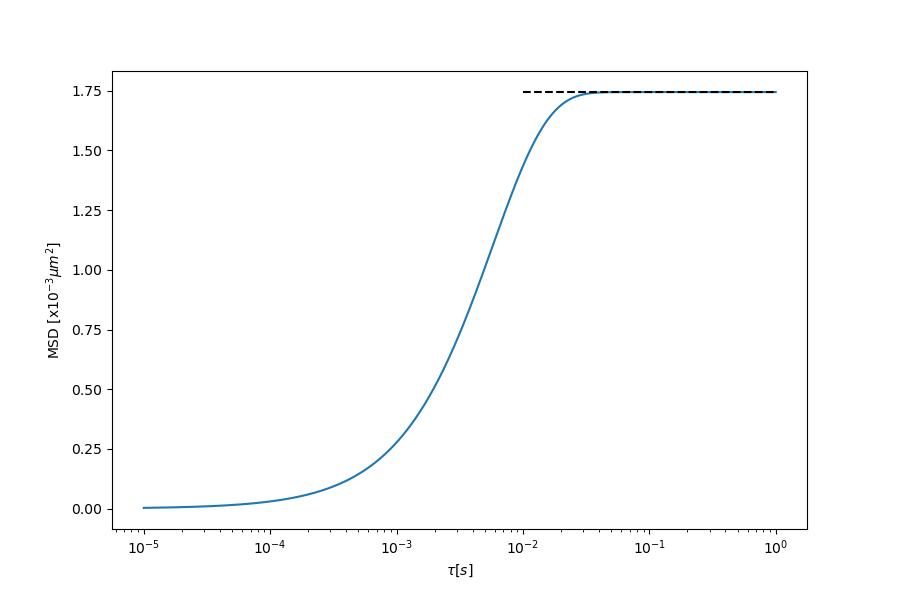
\includegraphics[width=0.67\linewidth]{MSD.png}
	\caption{Example mean squared displacement using eq.~\ref{eq:MSD}, for a $1\mu m$ sphere trapped by an optical potential well. The dotted line represents the upper limit of the sphere's displacement due to the optical trap.}
\end{figure}
The MSD plot can be subdivided into two regimes, when $\tau \gg \tau_{OT}$ the particle is experiencing the harmonic potential described by the equipartition theorem, and when $\tau \ll \tau{OT}$ the particle is said to be freely diffusing within the trap focus. Of course for a freely diffusing object the MSD will never reach a plateau value, comparing MSD's for different particles provides a simple visual indicator of the difference in trapping strength. The MSD method is an already very versatile analytical tool for diffusive motion, however it is rather slow in computing time meaning it is only really beneficial when a high degree of accuracy is required and shorter time resolutions are unavailable - such as using a quadrant photo diode instead or a high speed CCD.

\subsubsection{Angular Mean Square Displacement (MSAD)}
It is also possible to plot the angular MSD (MSAD) using simulative data, however there is yet to be a analytical expression for the MSAD of a freely diffusing particle. Vigilante \textit{et al} \cite{Vigilante2020} derived the upper limit of a dimer's MSAD along its long axis by assuming it was strongly trapped and so had limited angular motion, there expression gives:
\begin{align}
	\lim_{\tau\to\infty}\left<(\Delta u_z)^2\right> = 
	2\left[1-\frac{1}{4\beta\kappa_r} 
	\left(\frac{exp(\beta\kappa_r)-1}
	{exp(\beta\kappa_r)F(\sqrt{\beta\kappa_r})
	}\right)^2\right]
\end{align}  
Vigilante's paper expressed that they couldn't compute $MSD(\tau)$ because they couldn't solve the Einstein-Smoluchowski equation which describes the diffusion constant for dielectric particles. This would require a full description of a particle's electrical mobility and charge distribution - the latter could be achieved via a discrete dipole approximation, the former would be dependent on both the particle's position but relative orientation to the electric field.

\subsection{Power Spectrum Density (PSD)}
The power spectral density (PSD) method is by far the most versatile method for observing the dynamics of any object within an optical trap, allowing for fast calibration times while also quickly filtering out typical noise sources. Taking the Fourier transform of a particle's trajectory yields:
\begin{align}
	\hat{x}(f) = \frac{(2D)^{1/2}\hat{\eta}}{2\pi(f_c-if)}
\end{align}
where $\hat{\eta}$ is the Fourier transform of the white noise, where the values are exponentially distributed as opposed to being normally distributed in the time domain \cite{BergSoerensen2004}, the correlation function is given as:
\begin{align}
	\left<\hat{\eta_k}\hat{\eta_l^*}\right> = t_{msr} \delta_{k,l} \rightarrow \left< \eta^4 \right> = 2t_{msr}
\end{align} 
We can therefore ignore the white noise from our analysis by looking at the spectral density of $\hat{x}(f)$: 
\begin{align}
	\label{eq:lorentzian}
	S_x = \frac{\hat{x}^2}{t_{msr}} = \frac{D}{2\pi(f_c^2+f^2)}
\end{align}
We can fit the Lorentzian via a simplified geometric series $S_x = 1/(A+Bf_k^2)$ which allows us to compute both the diffusion coefficient (in arbitrary units) and the corner frequency $f_c$ which is directly related to the trap strength via $f_c = \kappa_x/(2\pi\gamma)$. Like with the analytical expression of the mean squared displacement we see two distinct regions, when $f\ll f_c$ the PSD reaches a plateau value that when converted to length units represents the maximum displacement the particle can move beyond the focus, however when $f\gg f_c$ the PSD falls off exponentially which denotes the particle is freely diffusing within the beam focus.
\begin{figure}[t]
	\centering
	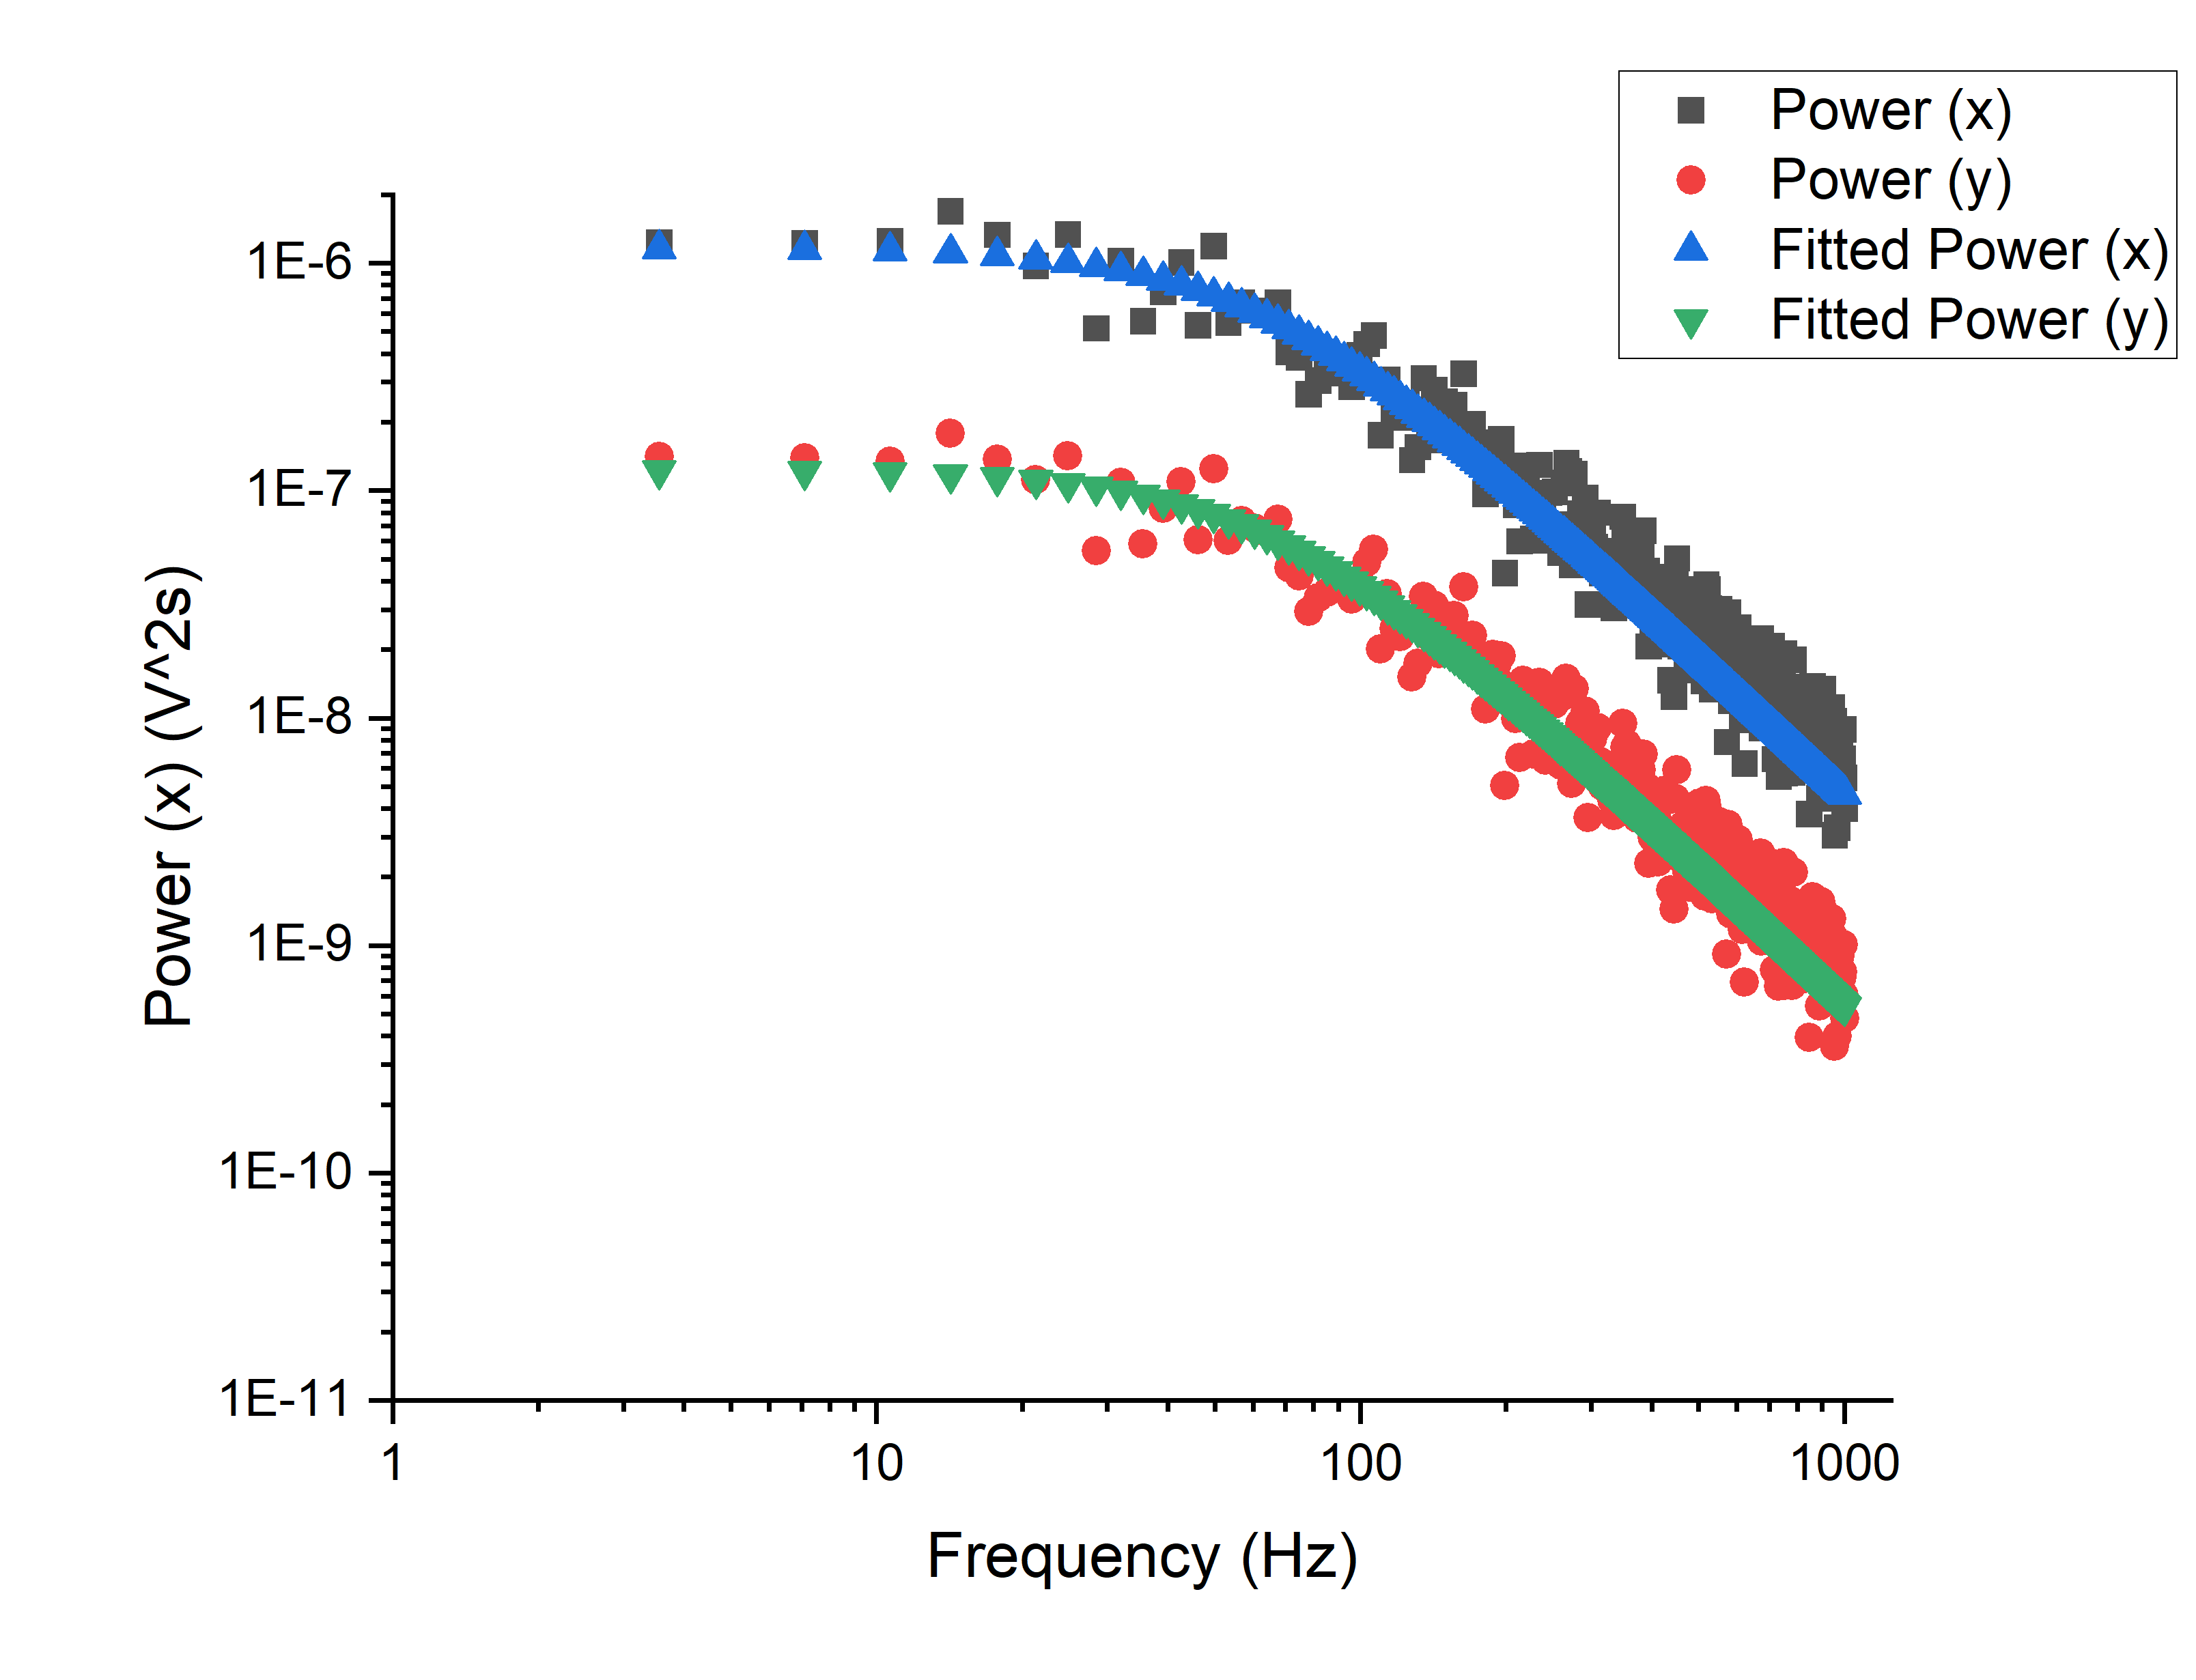
\includegraphics[width=0.75\linewidth]{PSD.png}
	\caption{Example PSD fitted using Eq.~\ref{eq:lorentzian}, power spectra is collected from an optically trapped silica sphere suspended in water. The difference in magnitude is due to the asymmetry of the quadrant photo diode having a stronger signal response in the direction of the polarisation vector. Using a correction factor (see Eq.~\ref{eq:correction_factor}) will adjust the power spectra to better describe the trap shape.}
\end{figure}
The Lorentzian relationship is only valid for frequency terms up to the Nyquist frequency (half of our sampling rate), this is because we are only taking a finite sampling of the particle's trajectory meaning the signal is aliased. Berg and Sorensen provide a suitable modified Lorentzian to account for the aliasing effects \cite{BergSoerensen2004}:
\begin{align}
	S_x = \frac{(\Delta x)^2\Delta t}{1+c^2-2c\cos{2\pi f_k\Delta t/N}}
\end{align}
Where N is the total number of samples taken, $\Delta x \ \& \ c$  have no direct physical interpretation and are defined in \cite{BergSoerensen2004}. Further modifications can be made to the power spectrum model but this is only useful when a high degree of accuracy is necessary. Typically power spectra are recorded using a Quadrant Photo Diode (QPD), which records motion in voltage units, not in units of length. To convert between the two we have a few methods: Firstly if we have a mono-disperse suspension of particles, the laser can be scanned across the surface of our target particle; so long as the particle's size is known a linear conversion factor can be used to convert from voltage to length units. Secondly, if the size distribution is very wide but each particle can be accurately sized, then a conversion factor can be approximated by comparing the fitted value of the diffusion coefficient, and the reported value given by the Stokes-Einstein relation.

\begin{align}
	\label{eq:correction_factor}
	D_{SE} = \frac{k_BT}{\gamma_0} \Rightarrow Conversion\ Factor \ [m/V]= \sqrt{\frac{D_{SE}}{D_{fit}}}
\end{align}

With the latter method, the local fluid viscosity must be known to a high degree of accuracy, depending on the local heating effect this may be as trivial increase or it may be significant enough to drastically alter the characterisation. PSD analysis is often seen as the gold standard for calibration as it can be fine tuned to the point that optical forces can be computed on the order of $10^{-15} N$ \cite{BergSoerensen2004}, it captures all of the information acquired by other calibration techniques while filtering out noise and requiring a relatively small amount of data collected. 

\section{Simulation of spherical aggregates}
Later chapters cover the dynamics of spherical aggregates and anisotropic scatterers, these subjects are particularly difficult to characterise using conventional calibration techniques \cite{Li2008, Yogesha2011PreciseCO}. As an example consider a symmetric dimer as a paradigmatic aggregate; if we consider the Langevin equation for such a aggregate within an optical trap we have:
\begin{align}
	\frac{\mathbf{d}\vec{r}(t)}{\mathbf{dt}} = \frac{\vec{\kappa}_x}{\gamma}\vec{r}(t) + \sqrt{2\vec{D}_x}\eta(t)
\end{align}
Where $x(t)$ is replaced with $\vec{r}(t)$ to signify that the translational motion is generalised to a 3 dimensional case. Except now, the dimer is undergoing random rotational motion in addition to its Brownian translational motion the first term on the right hand side is no longer purely a function of the dimer's position but also on its orientation. The rotational form of the Langevin equation for a dipole within an external potential is given as:
\begin{align}
	\frac{\mathbf{d}\vec{u}(t)}{\mathbf{dt}} = \frac{\mu}{\gamma_R}\left[\vec{u}(t)\times E(t)\right]\times \vec{u}(t) + \sqrt{2\vec{D}_R}\lambda(t)\times \vec{u}(t)
\end{align}
Where $\vec{u}(t)$ is the unit vector aligned along the centres of the two spheres, $\mu$ is its dipole moment, and $\gamma_R$ is the rotational friction coefficient which is given as $\gamma_R = 8\pi\eta r^3$, if the dimer is within a harmonic potential we can write the first term on the right hand side as $\frac{\vec{\kappa}_u}{\gamma} \times \vec{u}(t)$, where $\vec{\kappa}_u$ is the rotational stiffness vector. $\lambda(t)$ is the Brownian rotations from the surrounding fluid, like in the translational case the Brownian rotations are normally distributed and are also uncorrelated so that:
\begin{align}
	\left<\lambda(t)\lambda(t')\right> = \delta_{ij}\delta(t-t')
\end{align}
For an asymmetric scatterer whose radius is comparable to that of the electric field's wavelength we now have a system of simultaneous equations:
\begin{align}
	\label{eq:full_langevin}
		\frac{\bold{d}\vec{r}(t)}{\bold{dt}} &= \frac{\vec{\kappa}_x(\vec{u}(t))}{\gamma}\vec{r}(t) + \sqrt{2D}\eta(t) \\
		\frac{\bold{d}\vec{u}(t)}{\bold{dt}} &= \frac{\vec{\kappa}_u(\vec{r}(t))}{\gamma_R}\times \vec{u}(t) + \sqrt{2\vec{D}_R}\lambda(t)\times \vec{u}(t)
\end{align}
Fortunately, we do not need to solve these directly as the latter two random variables can be easily approximated if the thermal energy of the system is know, and the rate of change can be assumed as linear if we take a sufficiently small time step that $\Delta t~\ll~\kappa_x/\gamma \ \& \ \Delta t \ll \kappa_u/\gamma_R$. In doing so we now only need to compute the optical force and torque applied to our dimer, this has already been compiled in a MATLAB package called \textit{Optical Tweezer Toolbox} or \textit{ott} \cite{Nieminen2007}. In which they use the results from \cite{Farsund1996} to compute both the optical force and torque using the beam coefficients - the form given by \cite{Crichton2000THEMD} is an easier form to compute: 
\begin{equation}
\begin{split}
	\bold{F_z}=&-\frac{1}{4\pi k^2}\sum_{n,m} \left(\frac{m}{n(n+1)}\Im[a_{n,m}b*_{n,m}-p_{n,m}q*_{n,m}] \right. \\ 
	&+\frac{1}{n+1}\left[\frac{n(n+2)(n-m+1)(n+m+1)}{(2n+1)(2n+3)} \right]^{1/2}  \\
	& \left. \times \Im[b_{n,m}b*_{n,m}+a_{n,m}a*_{n+1,m} - q_{n,m}q*_{n,m}+p_{n,m}p*_{n+1,m}] \right)
\end{split}
\end{equation}
\begin{equation}
\begin{split}
	\bold{T_z}=&-\frac{1}{8\pi k^3}\sum_{n,m} \left(\frac{m}{n(n+1)}[|a_{n,m}|^2+|b_{n,m}|^2-|p_{n,m}|^2-|q_{n,m}|^2] \right. \\ 
	&+\frac{2}{n+1}\left[\frac{n(n+2)(n-m+1)(n+m+1)}{(2n+1)(2n+3)} \right]^{1/2}  \\
	& \left. \times \Re[b_{n,m}a*_{n,m}+a_{n,m}b*_{n+1,m} - p_{n,m}q*_{n,m}+q_{n,m}p*_{n+1,m}] \right)
\end{split}
\end{equation}
Where $a_{n,m}$, $b_{n,m}$, $p_{n,m}$ $q_{n,m}$ are the beam coefficients of the incident and scattered fields respectively. We can get the transverse force and torque components in a similar form by applying a simple rotation transformation. In order to get the scattered beam coefficients we can use \textit{MSTM} \cite{Mackowski2011} to calculate the T-matrix of our dimer (or any spherical aggregate). Vigilante et al compiled together a python package that combines both \textit{ott} and \textit{MSTM} to simulate the behaviour of spherical aggregates within a predefined optical trap. 

Throughout this PhD we use the work of Vigilante to perform a systematic study of the dynamics demonstrated by asymmetric dimers in both plane and circularly polarised light. But furthermore we expand upon their work to create a fully functional quadrant photo-diode to simulate the response from a calibration test. This builds upon the work from \cite{Rohrbach2002} which applied the fundamental principles of Lorenz-Mie theory to replicate the response signal of a QPD being used in back focal-plane interferometry.

\subsection{Simulated Quadrant Photodiode}
In order to simulate a typical experimental set up with a QPD installed as a position detection system we need to evaluate the total magnitude of the electric field incident on the photo-diode surface. While trapping a micro-particle, the scattered and incident fields combine together and interfere with one another. These fields are collected by a condenser lens in the far field limit and are focused onto the QPD surface, the total intensity can be evaluated as:
\begin{align}
I(x,y) = \epsilon_0c\left|
\begin{bmatrix} 
	E_{i,x}(x,y)+E_{s,x}(x,y) \\ 
	E_{i,y}(x,y)+E_{s,y}(x,y) \\ 
	E_{i,z}(x,y)+E_{s,z}(x,y)
\end{bmatrix} \right|^2 \times step(NA_c-\sqrt{x^2+y^2})
\end{align}
The last term is simply a representative step term that defines the outer limit by which we evaluate the electric field, this is analogous to our condenser lens removing noise from other light sources by only accepting light at a specific acceptance angle defined by its numerical aperture $NA_c$. Depending on the relative size of our particle we can adjust the acceptance angle, this has very little effect on the transverse signals, but for axial evaluations of a trapped particle the numerical aperture should be tuned so that the resultant response curve has negative slope in order to allow for axial position detection, the method for finding this angle $\theta_\Theta$ is discussed in \cite{Friedrich2012}.

The incident beam is simple enough to define given our set up parameters, for the sake of simplicity we assume that our beam is a Laguerre-Gaussian beam of mode $[0.0, 0.0]$ (which is simply a pure Gaussian beam). \textit{Ott} uses a point matching approach to approximate the beam shape coefficients of the incident field by fitting it to the far field estimate, the beam is of the form:

\begin{align}
	E_{inc}(kr)=\sum^\infty_n\sum^n_{m=-n}a_{mn}RgM_{nm}(kr)+b_{nm}RgN_{nm}(kr)
\end{align}

Where $RgM_{nm}(kr)$ \& $RgN_{nm}(kr)$ are regular vector spherical wave functions, \textit{ott} allows us to change the basis of the the incident beam to suit our needs, because we are measuring in the far field we want to set our incident beam to be an outgoing spherical wave so that we can compute the intensity on the QPD. For spherical waves the field can either be expressed as an incoming/outgoing wave (with a singularity at the origin) or as a regular wave around the origin; for incoming/outgoing waves the wave functions use the first/second forms of the Hankel function respectfully. In order to compute the regular spherical wave at the origin we replace the Hankel function with the Bessel function which is simply the average of the first and second forms of the Hankel function, so at the origin we avoid a singularity of the EM field.  

We can if we want further restrict the incident beam by applying setting the truncation angle to match our microscope object, this essentially applies a cut off point to the In order to compute the scattering from the target particle \textit{ott} uses the t-matrix method, this is not essential for a simple sphere but is essential for complex shaped particles such as dimers. The scattered and incident fields are then combined

\begin{figure}
	\centering
	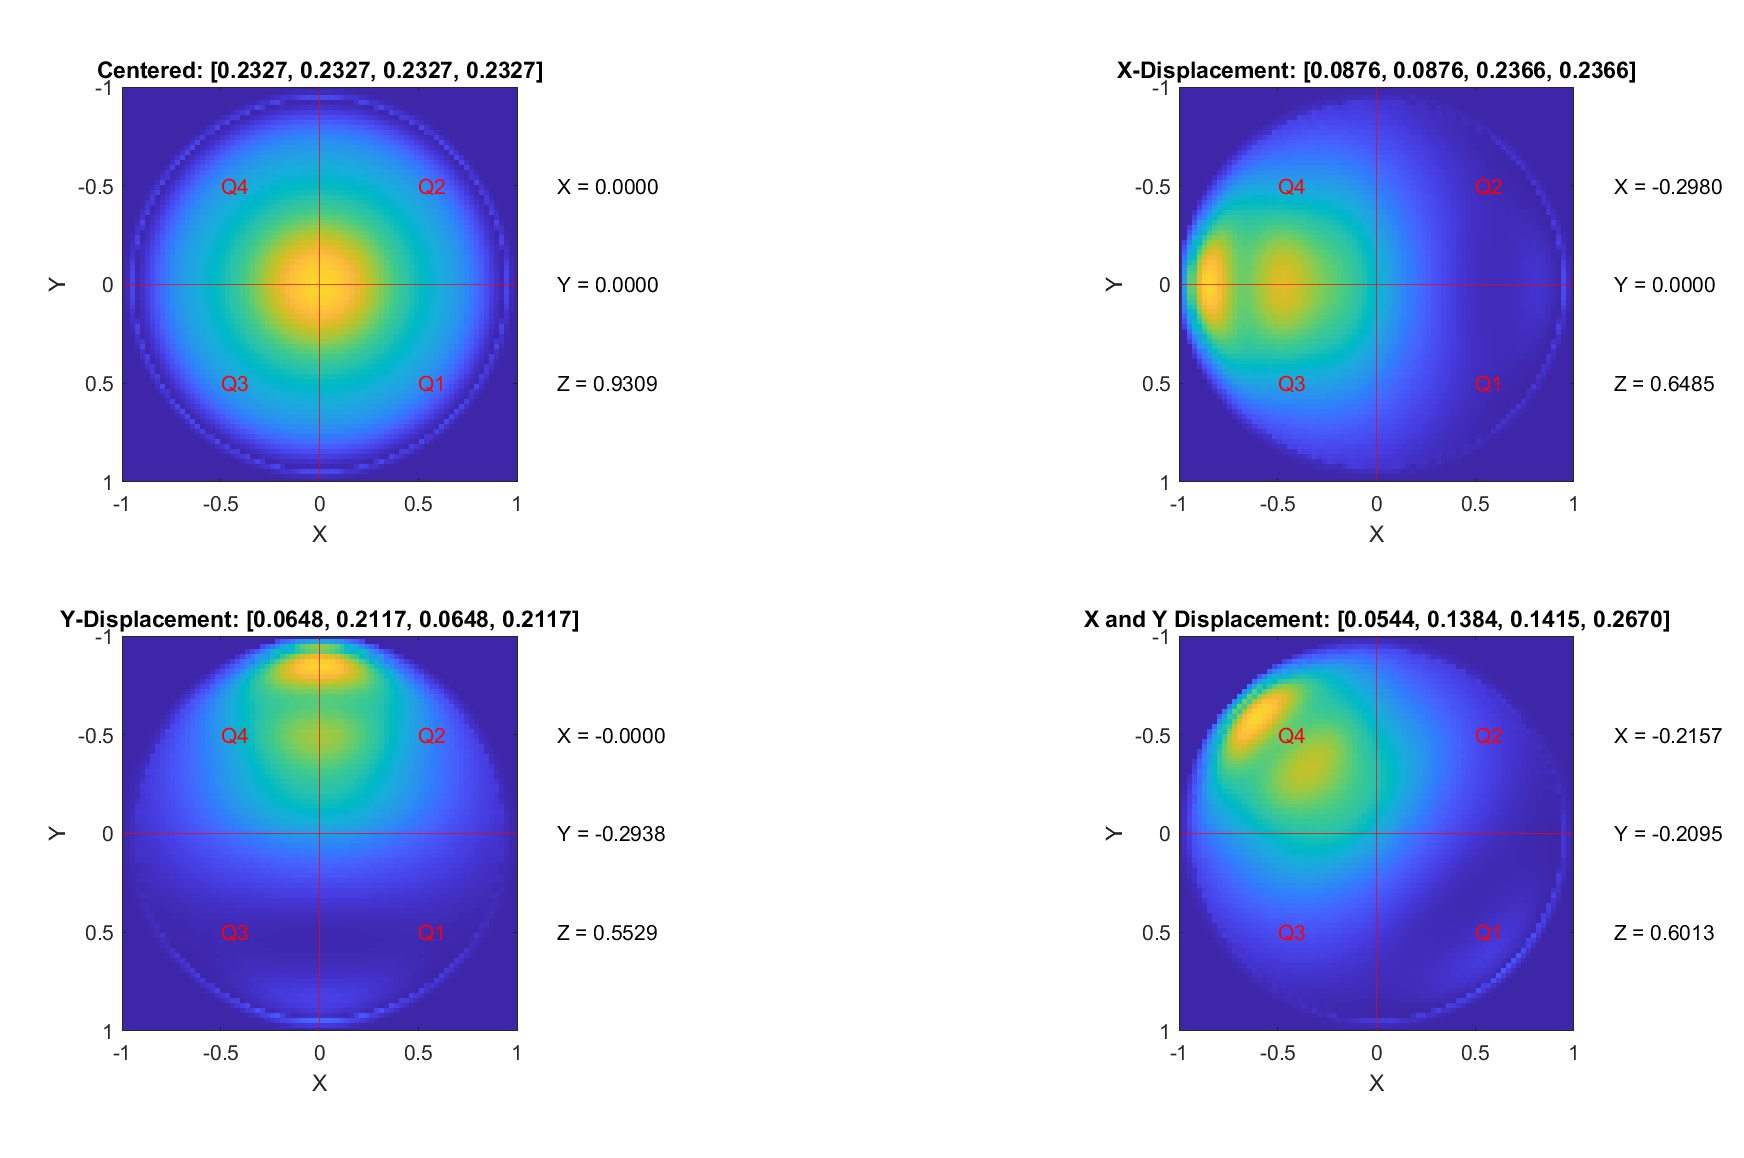
\includegraphics[width=0.75\linewidth]{fixed_polarisation.png}
\end{figure}
